\documentclass[tikz,border=2mm]{standalone}
\usepackage{tikz}
\usetikzlibrary{shapes,arrows,positioning}

\begin{document}
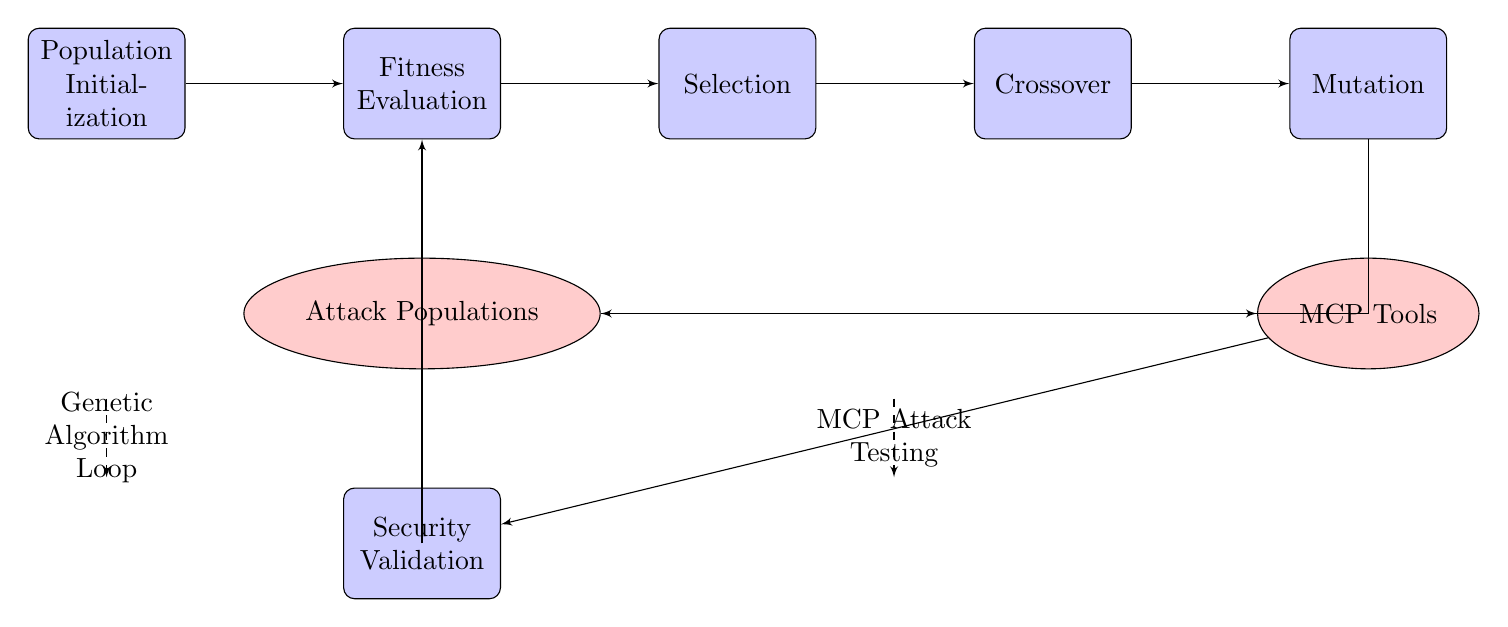
\begin{tikzpicture}[
    block/.style={rectangle, draw, fill=blue!20, text width=5em, text centered, rounded corners, minimum height=4em},
    line/.style={draw, -latex'},
    cloud/.style={ellipse, draw, fill=red!20, minimum height=4em}
]

    % Genetic Algorithm Components
    \node [block] (init) {Population Initialization};
    \node [block, right=2cm of init] (fitness) {Fitness Evaluation};
    \node [block, right=2cm of fitness] (selection) {Selection};
    \node [block, right=2cm of selection] (crossover) {Crossover};
    \node [block, right=2cm of crossover] (mutation) {Mutation};

    % Semantic Attack Generation Flow
    \node [cloud, below=1.5cm of fitness] (attack) {Attack Populations};
    \node [cloud, below=1.5cm of mutation] (mcp) {MCP Tools};
    \node [block, below=1.5cm of attack] (validation) {Security Validation};

    % Connections
    \path [line] (init) -- (fitness);
    \path [line] (fitness) -- (selection);
    \path [line] (selection) -- (crossover);
    \path [line] (crossover) -- (mutation);
    \path [line] (mutation) |- (attack);
    \path [line] (attack) -- (mcp);
    \path [line] (mcp) -- (validation);
    \path [line] (validation) -| (fitness);

    \node [text width=5em, text centered] at (0,-4.5) {Genetic Algorithm Loop};
    \node [text width=6em, text centered] at (10,-4.5) {MCP Attack Testing};
    \path [line, dashed] (0,-4) -- (0,-5);
    \path [line, dashed] (10,-4) -- (10,-5);

\end{tikzpicture}
\end{document}